% !TEX program = xelatex
% Progress Review — 8 June 2026
% Vibe Networking: Network Engineering (YBL1)

\documentclass[11pt,aspectratio=169]{beamer}

% ── Packages ─────────────────────────────────────────────────────────────────
\usepackage{fontspec}
\usepackage{tikz}
\usepackage{listings}
\usepackage{booktabs}
\usepackage{array}
\usepackage{xcolor}

% ── Theme ────────────────────────────────────────────────────────────────────
\usetheme{Madrid}
\usefonttheme{professionalfonts}

% ── Metadata ─────────────────────────────────────────────────────────────────
\title[Progress Review]{Vibe Networking --- Network Engineering}
\subtitle{Progress Review}
\author[Student]
       {Student\\[4pt]
        \small Vibe Networking --- Network Engineering}
\date{8 June 2026}
\institute{Information Engineering Final Year Project}

% ── Code listing style ───────────────────────────────────────────────────────
\lstset{
  basicstyle=\tiny\ttfamily,
  breaklines=true,
  frame=single,
  language=Java,
  showstringspaces=false,
}

\begin{document}

% ══════════════════════════════════════════════════════════════════════════════
% Slide 1: Title
% ══════════════════════════════════════════════════════════════════════════════
\begin{frame}
  \titlepage
\end{frame}

% ══════════════════════════════════════════════════════════════════════════════
% Slide 2: Outline
% ══════════════════════════════════════════════════════════════════════════════
\begin{frame}{Outline}
  \tableofcontents
\end{frame}

% ══════════════════════════════════════════════════════════════════════════════
\section{Project Overview}
% ══════════════════════════════════════════════════════════════════════════════

\begin{frame}{Project Overview}
  \textbf{YBL1: Vibe Networking -- Network Engineering}

  \vspace{8pt}
  \textbf{Three Core Goals}:
  \begin{enumerate}
    \item Build an \textbf{LLM benchmark} for network configuration tasks.
    \item Identify LLM limitations in network configuration and explore
          \textbf{improvement strategies} (RAG, multi-agent, verification loop).
    \item Explore \textbf{LLM-driven automated network troubleshooting}.
  \end{enumerate}

  \vspace{8pt}
  \textbf{Platform}: Cisco Modeling Labs (CML) + MCP Server + OpenAI Agents SDK.
\end{frame}

% ══════════════════════════════════════════════════════════════════════════════
\section{Materials Studied}
% ══════════════════════════════════════════════════════════════════════════════

\begin{frame}{Materials Studied: LLM API \& Agent Harness}
  \textbf{Goal}: Acquire the knowledge to program an LLM via its API.

  \vspace{6pt}
  \begin{itemize}
    \item \textbf{OpenAI Agents SDK} --- tool-calling loop, agent lifecycle,
          conversation context management.
    \item \textbf{DeepSeek V4 Flash} --- primary LLM provider via
          OpenAI-compatible API; can switch to OpenAI GPT-4.1-mini in production.
    \item \textbf{MCP (Model Context Protocol)} --- JSON-RPC over stdio,
          enabling LLM-tool interoperability.
    \item \textbf{Agent Harness}: CLI $\to$ Runner $\to$ Agent $\to$ MCP Server
          $\to$ CML API.
  \end{itemize}

  \vspace{6pt}
  \textbf{Outcome}: Phase 1 agent harness completed (read-only mode).
\end{frame}

\begin{frame}{Materials Studied: Cisco Routing \& Literature}
  \textbf{Cisco Routing (IERG4090 Notes)}:
  \begin{itemize}
    \item Static routing, IP addressing, subnetting
    \item OSPF, EIGRP, RIP --- interior routing protocols
    \item BGP --- exterior gateway protocol
  \end{itemize}
  \small Target knowledge level: CCNP Route.

  \vspace{8pt}
  \textbf{Literature Review} (\texttt{research/literature-review.md}):
  \begin{itemize}
    \item \textbf{NetConfEval} (CoNEXT 2024): GPT-4 error-free in only
          $1/3$ of OSPF/RIP/BGP config runs without RAG.
    \item \textbf{NetConfBench} (IETF NMRG Draft): 40 JSON-defined tasks,
          three evaluation metrics (reasoning, command, testcase).
    \item \textbf{Cornetto} (ETH Zurich, 2026): LLMs frequently introduce
          regressions during troubleshooting; formal verification is essential.
  \end{itemize}
\end{frame}

% ══════════════════════════════════════════════════════════════════════════════
\section{Findings \& Progress}
% ══════════════════════════════════════════════════════════════════════════════

\begin{frame}{Progress: Agent Architecture}
  \centering
  \begin{tikzpicture}[
      node distance=1.8cm,
      box/.style={draw, rounded corners, minimum width=2.4cm, minimum height=0.8cm, align=center, fill=blue!10},
      arrow/.style={->, >=stealth, thick}
    ]
    \node[box] (cli) {CLI\\\texttt{java -jar ... run}};
    \node[box, right=of cli] (runner) {Runner\\task orchestration};
    \node[box, right=of runner] (agent) {Agent\\tool-calling loop};
    \node[box, right=of agent] (mcp) {MCP Server\\stdio JSON-RPC};
    \node[box, above=of mcp] (compat) {\texttt{\_cml\_compat.py}\\\small CML 2.7 compat layer};
    \node[box, right=of mcp] (cml) {CML API\\\small 2.7.2};

    \draw[arrow] (cli) -- (runner);
    \draw[arrow] (runner) -- (agent);
    \draw[arrow] (agent) -- (mcp);
    \draw[arrow] (compat) -- (mcp);
    \draw[arrow] (mcp) -- (cml);

    \node[below=0.6cm of agent, align=center, font=\footnotesize] {DeepSeek V4 Flash\\or OpenAI GPT-4.1-mini};
    \node[below=0.6cm of runner, align=center, font=\footnotesize] {Run Log\\\texttt{experiments/runs/}};
  \end{tikzpicture}

  \vspace{4pt}
  \begin{center}
    \footnotesize Java 25 \quad$\cdot$\quad
    Spring Boot 4.1 \quad$\cdot$\quad
    MCP Java SDK + cml-mcp stdio
  \end{center}
\end{frame}

\begin{frame}{Progress: CML Integration}
  \textbf{Phase 1 Safety Boundary --- 8 Read-Only Tools}:

  \vspace{4pt}
  \begin{columns}[t]
    \begin{column}{0.5\textwidth}
      \textbf{Allowed}:
      \begin{itemize}
        \item \texttt{get\_cml\_information}
        \item \texttt{get\_cml\_status}
        \item \texttt{get\_cml\_labs}
        \item \texttt{get\_cml\_lab\_by\_title}
        \item \texttt{get\_nodes\_for\_cml\_lab}
        \item \texttt{get\_interfaces\_for\_node}
        \item \texttt{get\_all\_links\_for\_lab}
        \item \texttt{get\_console\_log}
      \end{itemize}
    \end{column}
    \begin{column}{0.5\textwidth}
      \textbf{Blocked}:
      \begin{itemize}
        \item Create / delete / wipe lab
        \item Start / stop nodes
        \item Configure devices
        \item Send CLI commands
        \item Packet capture
        \item User management
      \end{itemize}
    \end{column}
  \end{columns}

  \vspace{8pt}
  \textbf{Verified}: \texttt{doctor} all-green, 9/9 unit tests passing.
\end{frame}

\begin{frame}{Progress: Agent Demo}
  \textbf{Example Run}: \texttt{java -jar target/netagent-benchmark-0.1.0-SNAPSHOT.jar run "list all labs on CML"}

  \vspace{6pt}
  \begin{block}{Agent Output (excerpt)}
    \small
    \begin{tabbing}
      \textbf{CML Version}: \= \texttt{2.7.2+build.26} \\
      \textbf{Server Ready}: \> \texttt{Yes} \\
      \textbf{Total Labs}: \> \texttt{1} \\
      \textbf{Lab Name}: \> \texttt{Lab at Fri 23:08 PM} \\
      \textbf{State}: \> \texttt{STARTED} \\
      \textbf{Nodes}: \> \texttt{2} \\
    \end{tabbing}
  \end{block}

  \vspace{6pt}
  \begin{itemize}
    \item Agent successfully queries CML server via MCP tools.
    \item Run logs auto-generated in \texttt{experiments/runs/}
          (API keys and passwords sanitized).
    \item All 8 read-only tools tested and working.
  \end{itemize}
\end{frame}

\begin{frame}{Key Technical Challenge: CML 2.7 Compatibility}
  \textbf{Problem}: CML server runs \textbf{2.7.2}, but cml-mcp 0.28.0
  expects fields introduced in CML 2.8+.

  \vspace{4pt}
  \textbf{Solution}: \texttt{\_cml\_compat.py} --- declarative import-hook
  patching layer.

  \vspace{6pt}
  \begin{table}
    \footnotesize
    \begin{tabular}{llp{4.5cm}}
      \toprule
      \textbf{Model} & \textbf{Missing Field} & \textbf{Patch} \\
      \midrule
      SystemInformation & \texttt{allow\_ssh\_pubkey\_auth} & Default: \texttt{False} \\
      SystemInformation & \texttt{oui}                    & Default: \texttt{None} \\
      ComputeHealth     & \texttt{docker\_shim}            & Default: \texttt{None} \\
      Lab               & \texttt{effective\_permissions}  & Default: \texttt{None} \\
      \bottomrule
    \end{tabular}
  \end{table}

  \vspace{4pt}
  \textbf{Key lessons}:
  \begin{itemize}
    \item Pydantic v2 required-field sentinel is \texttt{PydanticUndefined}, not \texttt{Ellipsis}.
    \item Must patch \emph{schema definition} modules, not importing modules.
    \item Must use \texttt{PathFinder.find\_spec} to avoid meta\_path recursion.
  \end{itemize}
\end{frame}

% ══════════════════════════════════════════════════════════════════════════════
\section{Literature Review: Key Findings}
% ══════════════════════════════════════════════════════════════════════════════

\begin{frame}{Literature Review: Key Findings}
  \begin{table}
    \footnotesize
    \begin{tabular}{p{2.8cm}p{6.5cm}}
      \toprule
      \textbf{Finding} & \textbf{Detail} \\
      \midrule
      Low-level config errors &
        GPT-4 produces error-free output in only 1/3 runs on OSPF/RIP/BGP
        without RAG. \\
      Basic mistakes &
        IP addressing, subnet mask conversion --- fluent but wrong. \\
      Transitive conflicts &
        Cannot detect indirect contradictions (e.g.\ $s_1\to s_2$ +
        $s_2$ cannot reach). \\
      Scale degradation &
        Performance drops sharply as topology grows (20 $\to$ 754 nodes). \\
      Repair regression &
        LLMs introduce new errors when fixing misconfigurations. \\
      Multi-agent promise &
        ConfAgent, CoTNet --- specialized agents for conflict detection and
        formal synthesis show improved results. \\
      \bottomrule
    \end{tabular}
  \end{table}

  \vspace{4pt}
  \textbf{Implication}: Reliable LLM-powered network automation requires
  \textbf{iterative, closed-loop workflows guided by formal verification}.
\end{frame}

% ══════════════════════════════════════════════════════════════════════════════
\section{Proposed Next Steps}
% ══════════════════════════════════════════════════════════════════════════════

\begin{frame}{Next Steps: Phase 2 --- Cisco Routing Knowledge}
  \textbf{Timeline}: $\sim$2 weeks.

  \vspace{6pt}
  \begin{enumerate}
    \item \textbf{Deepen Routing Knowledge}:
          \begin{itemize}
            \item Study IERG4090 lecture notes systematically.
            \item Practice static routing, OSPF, BGP configurations on CML.
            \item Target: CCNP Route level proficiency.
          \end{itemize}
    \item \textbf{Build CML Labs}:
          \begin{itemize}
            \item Design small-scale routing topologies.
            \item Test manually: routing convergence, failover, troubleshooting.
          \end{itemize}
    \item \textbf{Literature Deep Dive}:
          \begin{itemize}
            \item Study NetConfEval benchmark methodology in detail.
            \item Reproduce existing benchmarks if feasible.
          \end{itemize}
  \end{enumerate}
\end{frame}

\begin{frame}{Next Steps: Phase 3 --- Benchmark \& Improvement}
  \begin{enumerate}
    \item \textbf{Design LLM Benchmark for Network Configuration}:
          \begin{itemize}
            \item Define task taxonomy (static route, OSPF, BGP, troubleshooting).
            \item Develop evaluation metrics: config correctness, reachability,
                  convergence time.
            \item Automate benchmark execution with CML APIs.
          \end{itemize}
    \item \textbf{Explore Improvement Strategies}:
          \begin{itemize}
            \item \textbf{RAG}: augment prompts with Cisco documentation.
            \item \textbf{Multi-agent}: decompose tasks into planning,
                  configuration, verification agents.
            \item \textbf{Verification loop}: validate outputs against
                  formal network models.
          \end{itemize}
    \item \textbf{Troubleshooting Exploration}:
          \begin{itemize}
            \item Synthesize misconfigured topologies as test cases.
            \item Evaluate LLM fault diagnosis accuracy and regression rate.
          \end{itemize}
  \end{enumerate}
\end{frame}

\begin{frame}{Timeline}
  \centering
  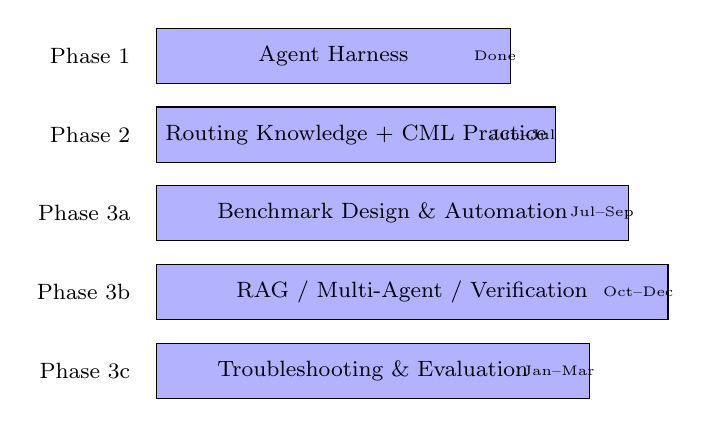
\begin{tikzpicture}[
      bar/.style={draw, fill=blue!30, minimum height=0.7cm, anchor=west},
      label/.style={font=\footnotesize, anchor=east}
    ]
    % Phase 1
    \node[label] at (0,0) {Phase 1};
    \node[bar, minimum width=4.5cm] at (0.2,0) {\footnotesize Agent Harness};
    \node[label, font=\tiny] at (4.9,0) {Done};

    % Phase 2
    \node[label] at (0,-1) {Phase 2};
    \node[bar, minimum width=5cm] at (0.2,-1) {\footnotesize Routing Knowledge + CML Practice};
    \node[label, font=\tiny] at (5.4,-1) {Jun--Jul};

    % Phase 3a
    \node[label] at (0,-2) {Phase 3a};
    \node[bar, minimum width=6cm] at (0.2,-2) {\footnotesize Benchmark Design \& Automation};
    \node[label, font=\tiny] at (6.4,-2) {Jul--Sep};

    % Phase 3b
    \node[label] at (0,-3) {Phase 3b};
    \node[bar, minimum width=6.5cm] at (0.2,-3) {\footnotesize RAG / Multi-Agent / Verification};
    \node[label, font=\tiny] at (6.9,-3) {Oct--Dec};

    % Phase 3c
    \node[label] at (0,-4) {Phase 3c};
    \node[bar, minimum width=5.5cm] at (0.2,-4) {\footnotesize Troubleshooting \& Evaluation};
    \node[label, font=\tiny] at (5.9,-4) {Jan--Mar};
  \end{tikzpicture}

  \vspace{12pt}
  \footnotesize Phase 3 dates are tentative; exact schedule subject to
  discussion with supervisor.
\end{frame}

% ══════════════════════════════════════════════════════════════════════════════
\section{Closing}
% ══════════════════════════════════════════════════════════════════════════════

\begin{frame}{Summary}
  \begin{itemize}
    \item \textbf{Phase 1 completed}: Agent harness with 8 read-only CML MCP
          tools, DeepSeek/OpenAI dual-provider support, run logging with
          secret sanitization.
    \item \textbf{CML 2.7 compatibility resolved}: declarative import-hook
          patching layer (\texttt{\_cml\_compat.py}) bridges schema gap.
    \item \textbf{Literature confirms}: LLMs alone are unreliable for network
          config; RAG, multi-agent, and formal verification are essential.
    \item \textbf{Next}: Phase 2 routing knowledge practice; Phase 3 benchmark
          design and improvement strategies.
  \end{itemize}

  \vspace{12pt}
  \begin{center}
    \large Thank you. Questions?
  \end{center}
\end{frame}

\end{document}
